\documentclass[cn,10pt,math=newtx,chinesefont=founder]{../elegantbook}

\title{力學題目彙整}
\subtitle{2021年}

\author{李宥頡}
\institute{National Taiwan University}
%\date{May 2, 2021}
%\version{4.1}
%\bioinfo{自定义}{信息}


\setcounter{tocdepth}{3}

%\logo{logo-blue.png}
\cover{cover.jpg}

% 本文档命令
\usepackage{array}
\newcommand{\ccr}[1]{\makecell{{\color{#1}\rule{1cm}{1cm}}}}

\definecolor{customcolor}{RGB}{32,178,170}
\colorlet{coverlinecolor}{customcolor}

\begin{document}

\maketitle
\frontmatter

\chapter*{序}
\tableofcontents

\mainmatter

\chapter{程力}
\section{斜拋}
拋體運動根據運動獨立性(或稱運動重疊原理),可將一曲線運動分為兩個正交方向的直線運動來討論。一般來說,習慣分解成水平方向與鉛直方向,以常見的直角笛卡爾
座標(Cartesian Coordinate),我們將水平方向稱為$x$方向,鉛直方向稱為$y$方向,由於重力恆指向$-y$,故鉛直方向作鉛直上拋運動,且水平方向不受重力,
故水平方向作等速度運動。根據上述,運動的含時參數方程(參數為時間$t$)為
\begin{equation}\label{1.1}
    x = v_0 \cos\theta t\ \ \ \ \ \ \ y = (v_0 \sin\theta)t -\frac{1}{2}gt^2
\end{equation}
\begin{equation}
    v_x = v_0 \cos\theta \ \ \ \ \ \ \ v_y = v_0 \sin\theta - gt
\end{equation}
對於斜拋來說,我們主要對飛行時間$T$、最大高度$H$、水平射程$R$有興趣。直覺上飛行時間應由鉛直方向決定,因為水平方向作等速度運動,看不出時間的影響,故
從鉛直方向的上拋運動判斷。由於上拋上下程的對稱性,飛行時間$T=T_{上}+T_{下}=2T_{上}=\frac{2v_0 \sin\theta}{g}=\frac{2v_{0y}}{g}$。
由於水平方向為等速度運動,水平射程$R = $水平初速 $\times T = \frac{2 v_0 \cos\theta \sin\theta}{g} = \frac{v_0 \sin 2\theta}{g}$。
最後,最大高度$H$由上拋得出,可得$H=\frac{v_0^2 \sin^2\theta}{2g}=\frac{v_{0y}^2}{2g}$。\\
\begin{equation}
\begin{array}{l}
    T = \frac{2v_0 \sin\theta}{g} \\
    R = \frac{v_0 \sin 2\theta}{g} \\
    H = \frac{v_0^2 \sin^2\theta}{2g}
\end{array}
\end{equation}
斜拋重點討論:
\begin{enumerate}
    \item 水平射程$R = \frac{v_0 \sin 2\theta}{g}$在初速$v_0$固定時,
          有一最大值$R_{Max}=\frac{v_0^2}{g}$,
          並發生在$\theta_{Max}=\frac{\pi}{4}$
    \item 同一水平射程$R = \frac{v_0 \sin 2\theta}{g}=\frac{2v_0 \sin \theta \cos \theta}{g}$,
          在固定初速度並透過簡單的代換可知,有兩個拋射角$\theta_1 , \theta_2$滿足同一射程,且
          \begin{equation} \label{1.4}
            \theta_1+\theta_2 = \frac{\pi}{2}
          \end{equation}
\end{enumerate}


\section{斜拋打斜面}
\subsection{運動方程}
在討論斜面上的斜拋運動,我們常選擇平行斜面方向為$x$軸,而垂直斜面方向為$y$軸。分解初速和加速度
之後,此時兩方向的運動均為等加速度運動。\\
\begin{minipage}{\linewidth}
    \begin{minipage}{0.45\linewidth}
\raggedleft
\flushleft
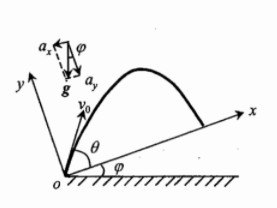
\includegraphics[width=0.5\textwidth]{image/斜拋打斜面.png}
    \end{minipage}
    \hspace{0.05\linewidth}
    \begin{minipage}{0.45\linewidth}
\raggedright
\begin{equation} \label{1.5}
    x = v_0 \cos\theta t\pm \frac{1}{2}(g \sin \varphi) t^2 \ \ \ \ \ \ \ y = (v_0 \sin\theta)t -\frac{1}{2}(g\cos \varphi) t^2
\end{equation}
\begin{equation}
    v_x = v_0 \cos\theta \pm (g \sin \varphi) t \ \ \ \ \ \ \ v_y = v_0 \sin\theta - (g\cos \varphi) t
\end{equation}
    \end{minipage}
\end{minipage}
若欲求斜拋打斜面的射程,即令方程式\ref{1.4}中的$y$為0,求出的$x$值即為射程$R$
\begin{equation}
    R = \frac{2v_0^2 \cos (\theta+\varphi)\sin \theta}{g\cos^2 \varphi}
\end{equation}
在固定$v_0$時,最大射程($+$為向上斜拋,$-$為向下斜拋)
\begin{equation}
    R_{Max}=\frac{v_0^2}{g(1\pm \sin \varphi)}
\end{equation}
和相對應的拋射角($-$為向上斜拋,$+$為向下斜拋)
\begin{equation}
    \theta_{Max} = \frac{\pi}{4} \mp \frac{\varphi}{2}
\end{equation}
\begin{proof}
    \\[20em]
\end{proof}

\begin{note}
    如何找三角函數極值:
    \begin{enumerate}
        \item 利用$\sin$,$\cos$的極值分別發生在$\frac{\pi}{2}$,$0$
        \item 利用三角疊合
        \item 利用和差化積、積化和差轉回1.
        \item 一次微分檢驗
    \end{enumerate}
\end{note}




\section{軌跡方程}
雖然運動方程(即位置與時間的函數關係)已經提供充足的解題要素,在實際處理問題上,
軌跡方程因為消去時間參數$t$,因此在解題上面對不含時的問題中,可以更清楚看到初速與
拋射角的關係。將方程 \ref{1.1}代換
\begin{equation}
    t = \frac{x}{v_0 \cos \theta}
\end{equation}
並代入$y$,即可獲得軌跡方程
\begin{equation}
    y=x \operatorname{tan} \theta-\frac{g x^{2}}{2 v_{0}^{2}\cos^2 \theta}
\end{equation}
利用三角恆等式
\begin{equation}
    1+\tan^2 \theta = \sec^2 \theta 
\end{equation}
代換的原因可以使軌跡方程中的角度,變成單一三角函數$\tan \theta$,方便後續討論
\begin{equation} \label{1.7}
    y=x \operatorname{tan} \theta-\frac{g x^{2}}{2 v_{0}^{2}}\left(1+\operatorname{tan}^{2} \theta\right)
\end{equation}
從方程式\ref{1.7}也可以側面證明出斜拋的確是數學上的拋物線$y = ax^2$,且二次項係數為負,代表開口朝下。
求出軌跡方程可幫助我們探討變數$x,y,v_0,\theta$之間的關係。\\
\begin{enumerate}
    \item 

若假定某斜拋的座標起點為原點$(0,0)$,並且在固定初速度$v_0$,並可通過點$(x, y)$,換句話說,方程
\ref{1.7}當中,只剩$\tan \theta$為變數,且可改寫成$\tan \theta$的二次函數
\begin{equation}
    \operatorname{tan}^{2} \theta-\frac{2 v_{0}^{2}}{g x} \operatorname{tan} \theta+\left(\frac{2 v_{0}^{2}}{g x^{2}} y+1\right)=0
\end{equation}
由二次函數的公式解,可求出$\tan \theta$
\begin{equation}
    \operatorname{tan} \theta=\frac{v_{0}^{2}}{g x} \pm \sqrt{\left(\frac{v_{0}^{2}}{g x}\right)^{2}-\left(\frac{2 v_{0}^{2}}{g x^{2}} y+1\right)}
\end{equation}
一般情況下,$\tan \theta$有兩解,且在斜拋的合理拋射角下(銳角),$\tan \theta$和$\theta$為一對一的函數關係,
即同一位置,在固定初速度之下,有兩個拋射角$\theta_1, \theta_2$對應到此位置,並且我們將證明,若此位置在斜面上
(斜角為$\varphi$),兩拋射角之間有關係(對應方程\ref{1.4},即是$\varphi = 0$的情形)
\begin{equation}
    \theta_1+\theta_2 = \frac{\pi}{2}+\varphi
\end{equation}
\begin{proof}
    \\[20em]
\end{proof}
    \item 在初速度和擊中點的$x$座標固定,最大高度$y_{max}$
    \begin{equation}
        y=y_{\max }=\frac{v_{0}^{2}}{2 g}-\frac{g x^{2}}{2 v_{0}^{2}}
    \end{equation}
    且拋射角$\theta_0$必滿足
    \begin{equation}
        \operatorname{tan} \theta=\operatorname{tan} \theta_{0}=\frac{v_{0}^{2}}{g x}
    \end{equation}
    \begin{proof}
        \\[20em]
    \end{proof}

\end{enumerate}
在斜拋打斜面問題中,主要可以分為兩種方法,第一種利用軌跡方程,解代數問題,此方法時常配合二次函數的
解,討論可行的拋射角。第二種方法是利用向量
\begin{equation}
    \vec{r} = \vec{v_0}t+\frac{1}{2}\vec{g}t^2 
\end{equation}
換句話說,位移向量總是$\vec{v_0}t$和$\frac{1}{2}\vec{g}t^2$兩向量做向量加法,
物理意義相當於先利用$v_0$作等速直線運動,再自由落體$\frac{1}{2}gt^2$,搭配斜面
的幾何,即可利用三角函數的正弦定律求解,見例題2-7。


\section{運動學練習題}

\begin{example}
    電梯以加速度1.22公尺/$秒^2$上升,當上升速度為2.44公尺/秒時,有一螺帽自電梯的天花板上鬆落,
    天花板與升降機的底面相距2.74公尺。請計算
    \begin{enumerate}
        \item 螺帽從天花板落到底面所需的時間
        \item 螺帽相對於電梯外固定柱子的位移和通過的路程
    \end{enumerate}

    \rightline{[練2-2]}
\end{example}
\newpage

\begin{example}
    卡車和汽車在同一車道上,前後均以等速前進,卡車的速度為$v_0$,後面汽車的速度為$3v_0$。由於霧大,能見度低,
    當汽車司機發現卡車時。兩車相距僅為$s_0$,汽車立即制動煞車。已知汽車制動煞車後等減速前進,須經距離$s_1$才
    能停止。試確定兩車不發生碰撞的條件。\\
    \rightline{[練2-3]}
\end{example}
\newpage

\begin{example}
    兩個相同的靜止小球A和B,質量均為$m$,A在B後的距離為a。如A受沿AB方向的沖量I的作用(方向沿AB方向),
    同時B受定力F(沿AB方向)開始運動。試確定A不超越B的條件。\\
    \rightline{[練2-4]}
\end{example}
\newpage

\begin{example}
    在同一起點,用相同大小的初速度以各不相同的拋射角拋出物體,求在同一鉛直面內各拋物線軌跡的最高點所組成的方程。\\
    \rightline{[練2-5]}
\end{example}    
\newpage

\begin{example}
    \begin{enumerate}
        \item 如圖所示,兩質點在地面上同一地點以相同速率$v_0$用不同拋射角$\alpha_1$和$\alpha_2$在同一鉛直面內拋出,作斜上拋運動。試證明
              當兩質點的射程$R$相同時,他們在空中飛行時間的乘積與射程$R$成正比,並忽略空氣阻力。
        \item 如圖所示兩質點在傾角為$\theta$的斜面底部同一位置,以相同的速率$v_0$用與斜面夾角$\alpha_1$和$\alpha_2$向斜面高處拋出,在同一鉛直面作
              斜上拋運動。試證明,當兩質點在斜面上射程$R$相同時,他們在空中飛行時間的乘積與斜面上射程$R$的關係。
        \item 試比較兩者的關係。
    \end{enumerate}
    \rightline{[練2-6]}
\end{example}
\begin{figure}[htbp]
    \flushright
    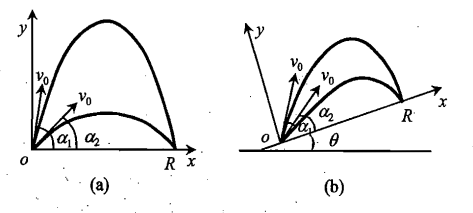
\includegraphics[width=0.3\textwidth]{image/prac_2_6.png}
\end{figure}
\newpage

\begin{example}
    如圖所示,高為$h$的旗竿頂端有一物$P$,一男孩在離旗竿底端A處距離$s$處的O點,欲用彈弓彈射小石塊擊中$P$。已知彈弓彈射出的小石塊初速度為$v_0$,
    問小石塊能擊中$P$的最小$v_0$為何?對應的彈射角應為多大(和水平線的夾角)?\\
    \rightline{[練2-7]}
\end{example}
\newpage

%題目2-8
\begin{example}
    足球運動員在距球門前方$s=11$米處的罰球點,準確地從球門正中橫梁邊沿下踢進一球。橫梁邊沿離地高度$h=2.5$米,足球質量為$m=0.5$千克,空氣阻力不計。求運動員至少要對足球做多少功?
    
    \rightline{[練2-8]}
\end{example}

\begin{solution}

\end{solution}




\newpage

%題目2-9
\begin{example}
    一斜面體兩斜面的傾角分別為$\theta$和$\varphi$,如圖2-練9(a)所示。一物體從傾角為$\theta$的斜面底角處做斜上拋運動。求為使物體從斜面體的頂角處切過,並落在傾角為$\varphi$的斜面底角處,則物體的拋射角$\alpha$與傾角$\theta$、$\varphi$應滿足什麼關係?(用簡單形式寫出。)
    
    \rightline{[練2-9]}
\end{example}

\begin{solution}

\end{solution}


\begin{figure}[htbp]
\flushright
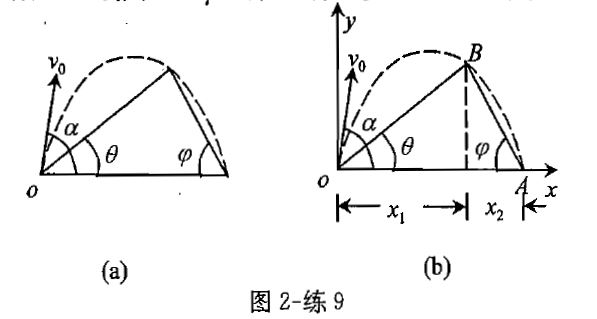
\includegraphics[width=0.5\textwidth]{image/2-9.jpeg}
\end{figure}

\newpage

%題目2-10
\begin{example}
    一輛汽車沿一圓周軌道以$v_0=7.0$米/秒的出速度作勻減速行駛。經過$t_1=5$秒後,汽車的加速度與速度之間的夾角$\theta_1=135^o$。又經過$t_2=3$秒後,其加速度與速度之間的夾角$\theta_2=150^o$。求:(1)圓軌道半徑R;(2)切向加速度的大小$a_\tau$;(3)這兩個時刻($t_1$和$t_1+t_2$時刻)的法向加速度$a_{n1}$和$a_{n2}$。
    
    \rightline{[練2-10]}
\end{example}

\begin{solution}
\begin{enumerate}[label=(\arabic*)]
    \item $R=62.5$米
    \item $a_\tau=0.40$米/秒$^2$
    \item $a_{n1}=0.40$米/秒$^2$,$a_{n2}=0.23$米/秒$^2$
\end{enumerate}
\end{solution}



\newpage

%題目2-11
\begin{example}
    一質點沿圓軌道由靜止開始作勻加速圓周運動。試求此質點的加速度與速度的夾角$\alpha$與其經過的那段圓弧對應的圓心角$\theta$之間的關係。
    
    \rightline{[練2-11]}
\end{example}

\begin{solution}
$tan\alpha=2\theta$
\end{solution}


\newpage

%題目2-12
\begin{example}
    一飛輪的角速度在5秒內由900轉/分均勻地減到800轉/分。求:(1)角加速度$\beta$;(2)在此5秒內的總轉數;(3)再經幾秒,輪將停止轉動。
    
    \rightline{[練2-12]}
\end{example}

\begin{solution}
\begin{enumerate}[label=(\arabic*)]
    \item 角加速度$\beta=-2.09$弧度/秒$^2$
    \item 總轉數$n=70.8$轉
    \item 40秒
\end{enumerate}

\end{solution}




\newpage

%題目2-13
\begin{example}
    有一半徑為R的剛性圓環豎直地在剛性水平地面上作純滾動,圓環中心以不變速度$v_0$在圓環平面內水平向前運動。求圓環上與圓心等高的P點的瞬時速度、切向加速度、法向加速度。如圖2-練13(a)所示。
    
    \rightline{[練2-13]}
\end{example}

\begin{solution}

\end{solution}


\begin{figure}[htbp]
\flushright
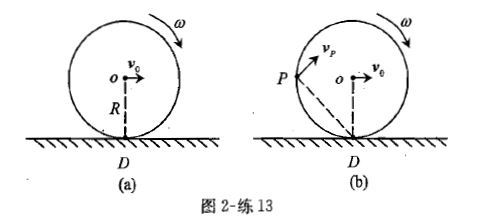
\includegraphics[width=0.6\textwidth]{image/2-13.jpeg}
\end{figure}

\newpage

%題目2-14
\begin{example}
    一質點在半徑為R的圓柱表面等螺距螺旋線上作等速率運動,已知此螺旋線的曲率半徑為$\rho$,質點在垂直於軸平面內的投影的運動週期為T,求質點作此螺旋線運動中沿軸方向的分速度為多大?
    \rightline{[練2-14]}
\end{example}

\begin{solution}

\end{solution}


\newpage

\begin{example}
    小球在豎直平面的 $O$ 點斜向上方拋出,拋射角為 $\theta$,速度大小為 $v_{0}$。
    在此豎直平面 內作 $O M$ 射線與小球拋射方向垂直,如圖 $1-9$ 所示. 小球到達 $O M$ 射線時的速率 
    $v$ 多大?\\
    \rightline{[舒1-4]}
\end{example}
\begin{solution}
    $v_{0} \sqrt{1+4 \cot ^{2} \theta}$
\end{solution}
\begin{figure}[htbp]
    \flushright
    \includegraphics[width=0.3\textwidth]{image/舒1-4.png}
\end{figure}
\newpage

\begin{example}
籃球比賽中,球不經碰撞直接進入籃圈,稱為空心入籃. 運動員在場內某處為使 球能空心入籃,
需要掌握球的拋射角 $\theta$ 和球的初速率 $v$. 實現空心籃的 $(\theta, v)$ 解並不唯一. 
引入最佳拋射角 $\theta_{0}$ (對應的初速率記為 $v_{0}$ ),意即在 $\theta_{0}$ 附近
運動員由於拋射角 $\theta_{0}$ 掌握不夠精確而產生小偏離量 $\Delta \theta$ 時
,為使球能空心入籃,需調整的 $v_{0}$ 偏移量 $\Delta v$ 為最小.某運動員站在 3 分線處立定投籃, 
3 分線與籃圈中心線間的水平距離為 $6.25 \mathrm{~m}$,籃圈離地高度 $3.05 \mathrm{~m}$, 
運動員投籃時出射點的高度為 2.23 $\mathrm{~m}$. 求最佳拋射角 $\theta_{0}$ 和對應的初速率 $v_{0}$.
\end{example}
\begin{solution}
    
\end{solution}


\chapter{隨手筆記}
\section{運動學}
時間的測量
\begin{enumerate}
    \item 測量$\pi$介子壽命,$\pi$介子在感光乳劑中產生並在其中留下細微的痕跡,用顯微鏡觀察,平均而言一個$\pi$
          介子在蛻變之前錒於走過了$10^-7 m$,且速度接近於光速,因此其壽命總共只有$10^-16 s$。(程力)
\end{enumerate}
\chapter{家教問題}
\section{力學}

\begin{example}
    如右圖,OD是水平面,AB和AC皆為斜面,斜角分別為$\theta_1 = 37^\circ$和$\theta_2 = 30^\circ$。一質點由A靜止,經斜面AB滑下,最後靜止於D,若
    改給予、一部為零的初速度$v_0$,經斜面AC滑下(斜面與平面皆有摩擦,且質點與接觸面間摩擦係數皆為$\mu$),則:
    \begin{enumerate}[label=(\Alph*)]
        \item 不論$v_0$為何,皆靜止於D點左側
        \item 不論$v_0$為何,皆靜止於D點右側
        \item 不論$v_0$為何,皆靜止於D點
        \item 若$\mu$同時變大,則必靜止於D點左側
        \item 若$\mu$同時變大,則必靜止於D點右側
    \end{enumerate}
\end{example}
























\end{document}